%definira klasu dokumenta 
\documentclass[12pt]{report} 

%prostor izmedu naredbi \documentclass i \begin{document} se zove uvod. U njemu se nalaze naredbe koje se odnose na cijeli dokument

%osnovni LaTex ne može riješiti sve probleme, pa se koriste različiti paketi koji olakšavaju izradu željenog dokumenta
\usepackage[croatian]{babel} 
\usepackage{amssymb}
\usepackage{amsmath}
\usepackage{txfonts}
\usepackage{mathdots}
\usepackage{titlesec}
\usepackage{array}
\usepackage{lastpage}
\usepackage{etoolbox}
\usepackage{tabularray}
\usepackage{color, colortbl}
\usepackage{adjustbox}
\usepackage{geometry}
\usepackage[classicReIm]{kpfonts}
\usepackage{hyperref}
\usepackage{fancyhdr}

\usepackage{float}
\usepackage{setspace}
\restylefloat{table}


\patchcmd{\chapter}{\thispagestyle{plain}}{\thispagestyle{fancy}}{}{} %redefiniranje stila stranice u paketu fancyhdr

%oblik naslova poglavlja
\titleformat{\chapter}{\normalfont\huge\bfseries}{\thechapter.}{20pt}{\Huge}
\titlespacing{\chapter}{0pt}{0pt}{40pt}


\linespread{1.3} %razmak između redaka

\geometry{a4paper, left=1in, top=1in,}  %oblik stranice

\hypersetup{ colorlinks, citecolor=black, filecolor=black, linkcolor=black,	urlcolor=black }   %izgled poveznice


%prored smanjen između redaka u nabrajanjima i popisima
\newenvironment{packed_enum}{
	\begin{enumerate}
		\setlength{\itemsep}{0pt}
		\setlength{\parskip}{0pt}
		\setlength{\parsep}{0pt}
	}{\end{enumerate}}

\newenvironment{packed_item}{
	\begin{itemize}
		\setlength{\itemsep}{0pt}
		\setlength{\parskip}{0pt}
		\setlength{\parsep}{0pt}
	}{\end{itemize}}




%boja za privatni i udaljeni kljuc u tablicama
\definecolor{LightBlue}{rgb}{0.9,0.9,1}
\definecolor{LightGreen}{rgb}{0.9,1,0.9}

%Promjena teksta za dugačke tablice
\DefTblrTemplate{contfoot-text}{normal}{Nastavljeno na idućoj stranici}
\SetTblrTemplate{contfoot-text}{normal}
\DefTblrTemplate{conthead-text}{normal}{(Nastavljeno)}
\SetTblrTemplate{conthead-text}{normal}
\DefTblrTemplate{middlehead,lasthead}{normal}{Nastavljeno od prethodne stranice}
\SetTblrTemplate{middlehead,lasthead}{normal}

%podesavanje zaglavlja i podnožja

\pagestyle{fancy}
\lhead{Programsko inženjerstvo}
\rhead{$<$Donor krvi$>$}
\lfoot{$<$Naziv grupe-dodat će se$>$}
\cfoot{stranica \thepage/\pageref{LastPage}}
\rfoot{\today}
\renewcommand{\headrulewidth}{0.2pt}
\renewcommand{\footrulewidth}{0.2pt}


\begin{document} 
	
	
	
	\begin{titlepage}
		\begin{center}
			\vspace*{\stretch{1.0}} %u kombinaciji s ostalim \vspace naredbama definira razmak između redaka teksta
			\LARGE Programsko inženjerstvo\\
			\large Ak. god. 2023./2024.\\
			
			\vspace*{\stretch{3.0}}
			
			\huge $<$Donor krvi$>$\\
			\Large Dokumentacija, Rev. \textit{$<$1.$>$}\\
			
			\vspace*{\stretch{12.0}}
			\normalsize
			Grupa: \textit{$<$Naziv grupe$>$}\\
			Voditelj: \textit{$<$Ime i prezime voditelja$>$}\\
			
			
			\vspace*{\stretch{1.0}}
			Datum predaje: \textit{$<$dan$>$. $<$mjesec$>$. $<$godina$>$.}\\
	
			\vspace*{\stretch{4.0}}
			
			Nastavnik: \textit{$<$Vlado Sruk$>$}\\
		
		\end{center}

	
	\end{titlepage}

	
	\tableofcontents


	\chapter{Dnevnik promjena dokumentacije}
		
		
		\begin{longtblr}[
				label=none
			]{
				width = \textwidth, 
				colspec={|X[2]|X[13]|X[3]|X[3]|}, 
				rowhead = 1
			}
			\hline
			\textbf{Rev.}	& \textbf{Opis promjene/dodatka} & \textbf{Autori} & \textbf{Datum}\\[3pt] \hline
			0.1 & Napravljen predložak.	& Ivan Smiljanić & 22.10.2023. 		\\[3pt] \hline 
			0.2	& Dodani opis projektnog zadatka, funkcionalni i nefunkcionalni zahtjevi & Ivan Smiljanić & 22.10.2023. 	\\[3pt] \hline 
			0.5 & Nadopunjavat će se s vremenom. & Ivan Smiljanić & 23.10.2023. \\[3pt] \hline 
			0.6 & Arhitektura i dizajn sustava, algoritmi i strukture podataka & * & 26.08.2013. \\[3pt] \hline 
			0.8 & Povijest rada i trenutni status implementacije,\newline Zaključci i plan daljnjeg rada & * & 28.08.2013. \\[3pt] \hline 
			0.9 & Opisi obrazaca uporabe & * & 07.09.2013. \\[3pt] \hline 
			0.10 & Preveden uvod & * & 08.09.2013. \\[3pt] \hline 
			0.11 & Sekvencijski dijagrami & * & 09.09.2013. \\[3pt] \hline 
			0.12.1 & Započeo dijagrame razreda & * & 10.09.2013. \\[3pt] \hline 
			0.12.2 & Nastavak dijagrama razreda & * & 11.09.2013. \\[3pt] \hline 
			\textbf{1.0} & Verzija samo s bitnim dijelovima za 1. ciklus & * & 11.09.2013. \\[3pt] \hline 
			1.1 & Uređivanje teksta -- funkcionalni i nefunkcionalni zahtjevi & * \newline * & 14.09.2013. \\[3pt] \hline 
			1.2 & Manje izmjene:Timer - Brojilo vremena & * & 15.09.2013. \\[3pt] \hline 
			1.3 & Popravljeni dijagrami obrazaca uporabe & * & 15.09.2013. \\[3pt] \hline 
			1.5 & Generalna revizija strukture dokumenta & * & 19.09.2013. \\[3pt] \hline 
			1.5.1 & Manja revizija (dijagram razmještaja) & * & 20.09.2013. \\[3pt] \hline 
			\textbf{2.0} & Konačni tekst predloška dokumentacije  & * & 28.09.2013. \\[3pt] \hline 
			&  &  & \\[3pt] \hline	
		\end{longtblr}
	
	
		\textit{Moraju postojati glavne revizije dokumenata 1.0 i 2.0 na kraju prvog i drugog ciklusa. Između tih revizija mogu postojati manje revizije već prema tome kako se dokument bude nadopunjavao. Očekuje se da nakon svake značajnije promjene (dodatka, izmjene, uklanjanja dijelova teksta i popratnih grafičkih sadržaja) dokumenta se to zabilježi kao revizija. Npr., revizije unutar prvog ciklusa će imati oznake 0.1, 0.2, …, 0.9, 0.10, 0.11.. sve do konačne revizije prvog ciklusa 1.0. U drugom ciklusu se nastavlja s revizijama 1.1, 1.2, itd.}
	\chapter{Opis projektnog zadatka}
		
		
    		Ovaj je projektni zadatak baziran na temi doniranja krvi. Ovom se aplikacijom doniranje   krvi nastoji automatizirati i dodatno olakšati te približiti potencijalnim donorima, ali i osobama koje dosad nisu donirale krvi te na taj način poboljšali sveukupno stanje i zalihe krvi. Na taj će se način automatizirati organiziranje doniranja krvi što će rezultirati boljom situacijom za kritične slučajeve. 
        	Prilikom samog pokretanja aplikacije, prikazat će se dostupna mjesta za doniranje krvi. Korisniku koji se nije registrirao, a želi vidjeti dostupna mjesta za doniranje krvi, bit će omogućeno tako što će se, odabirom na željeno mjesto, prikazati datum, mjesto i vrijeme organiziranih akcija doniranja krvi. Nadalje, neregistriranom korisniku bit će dostupne informacije o trenutno potrebnoj krvnoj grupi za odabrano mjesto. Korisniki koji se želi prijaviti u sustav bit će omogućeno prijaviti se s postojećim računom, uz pretpostavku da ga korisnik posjeduje, ili kreiranjem novog korisničkog računa za što će mu biti potrebno unijeti sljedeće podatke:
		\begin{packed_item}
			\item \textit{korisničko ime}
			\item \textit{lozinka}
			\item \textit{ime i prezime osobe}
			\item \textit{OIB}
			\item \textit{adresa}
			\item \textit{broj mobitela}
			\item \textit{email adresa osobe}
		\end{packed_item}
		
    		Registracijom korisnika u sustav, korisnik postaje potencijalni donor krvi. Nakon registracije, potencijalni donor može odabrati željenu lokaciju i rezervirati termin doniranja. Prije same rezervacije termina doniranja, korisnik mora potvrditi sustavu da se slaže s verificiranjem kritičnih podataka uporabom središnjeg informacijskog sustava primarne zdravstvene zaštite RH.\\
            \textbf{Donor} odabirom krvne grupe filtrira mjesta za doniranje krvi, prema potrebi, te na taj način popunjuje, odnosno rezervira, slobodno mjesto za doniranje. Nakon odlaska na mjesto doniranja krvi, korisnik se uvodi u evidenciju koja mu je dostupna u sustavu u bilo kojem trenutku. U slučaju da nema slobodnih mjesta za odabranu lokaciju doniranja krvi, sustav će pravovremeno obavijestiti korisnika te mu ponuditi alternativne lokacije. Osoba nije obvezna doći na rezerviran termin donacije krvi, međutim, popunjavanjem mjesta za doniranje krvi oduzima se mjesto potencijalnom donoru. Osoba u svakom trenutku može otkazati rezervaciju. Korisniku će na vrijeme biti poslan podsjetnik/obavijest kako bi na vrijeme mogao doći na termin ili kako bi znao postoji li potreba za donacijom. Registrirani korisnik može u svakom trenutku vidjeti svoju povijest doniranja kao i svoju medicinsku povijest.\\
            \textbf{Administrator} sustava verificira kritične podatke uporabom središnjeg informacijskog sustava primarne zdravstvene zaštite RH. Uloga je administratora administriranje stranice i registriranih korisnika kao i upravljanje bazom podataka te podacima samih korisnika. Administrator ima mogućnost ažuriranja lokacija za doniranje krvi, pristup povijesti donacija za svakog korisnika kao i pristup kritičnim podacima koje korisnik mora potvrditi. \\
            \textbf{Organizacije za prikupljanje krvi} redovito ažuriraju podatke o dostupnim zalihama krvi u svojim centrima putem aplikacije kako bi korisnici mogli vidjeti trenutnu dostupnost krvnih grupa. Osim toga, unose podatke i informacije o svojim centrima za darivanje krvi putem aplikacije što uključuje lokacije, radnom vremenu, kontaktu i slično. Također, organizacije mogu koristiti aplikaciju za komunikaciju s donatorima putem obavijesti o hitnim potrebama, podsjetnicima na donacije i zahvalama za njihovu podršku, a uz to mogu i planirati i organizirati donacije i promocije donatora.\\


            Dodat će se još naknadno s daljnom implementacijom
		\eject
		
		\section{IZBRISATI}
		
		\textit{Ovo potpoglavlje izbrisati.}\\

		U nastavku se nalaze različiti primjeri kako koristiti osnovne funkcionalnosti \LaTeX a koje su potrebne za izradu dokumentacije. Za dodatnu pomoć obratiti se asistentu na projektu ili potražiti upute na sljedećim web sjedištima:
		\begin{itemize}
			\item Upute za izradu diplomskog rada u \LaTeX u - \url{https://www.fer.unizg.hr/_download/repository/LaTeX-upute.pdf}
			\item \LaTeX\ projekt - \url{https://www.latex-project.org/help/}
			\item StackExchange za Tex - \url{https://tex.stackexchange.com/}\\
		
		\end{itemize} 	


		
		\noindent \underbar{podcrtani tekst}, \textbf{podebljani tekst}, 	\textit{nagnuti tekst}\\
		\noindent \normalsize primjer \large primjer \Large primjer \LARGE {primjer} \huge {primjer} \Huge primjer \normalsize
				
		\begin{packed_item}
			
			\item  primjer
			\item  primjer
			\item  primjer
			\item[] \begin{packed_enum}
				\item primjer
				\item[] \begin{packed_enum}
					\item[1.a] primjer
					\item[b] primjer
				\end{packed_enum}
				\item primjer
			\end{packed_enum}
			
		\end{packed_item}
		
		\noindent primjer url-a: \url{https://www.fer.unizg.hr/predmet/proinz/projekt}
		
		\noindent posebni znakovi: \# \$ \% \& \{ \} \_ 
		$|$ $<$ $>$ 
		\^{} 
		\~{} 
		$\backslash$ 
		
		
		\begin{longtblr}[
			label=none,
			entry=none
			]{
				width = \textwidth,
				colspec={|X[8,l]|X[8, l]|X[16, l]|}, 
				rowhead = 1,
			} %definicija širine tablice, širine stupaca, poravnanje i broja redaka naslova tablice
			\hline \SetCell[c=3]{c}{\textbf{naslov unutar tablice}}	 \\ \hline[3pt]
			\SetCell{LightGreen}IDKorisnik & INT	&  	Lorem ipsum dolor sit amet, consectetur adipiscing elit, sed do eiusmod  	\\ \hline
			korisnickoIme	& VARCHAR &   	\\ \hline 
			email & VARCHAR &   \\ \hline 
			ime & VARCHAR	&  		\\ \hline 
			\SetCell{LightBlue} primjer	& VARCHAR &   	\\ \hline 
		\end{longtblr}
		

		\begin{longtblr}[
				caption = {Naslov s referencom izvan tablice},
				entry = {Short Caption},
			]{
				width = \textwidth, 
				colspec = {|X[8,l]|X[8,l]|X[16,l]|}, 
				rowhead = 1,
			}
			\hline
			\SetCell{LightGreen}IDKorisnik & INT	&  	Lorem ipsum dolor sit amet, consectetur adipiscing elit, sed do eiusmod  	\\ \hline
			korisnickoIme	& VARCHAR &   	\\ \hline 
			email & VARCHAR &   \\ \hline 
			ime & VARCHAR	&  		\\ \hline 
			\SetCell{LightBlue} primjer	& VARCHAR &   	\\ \hline 
		\end{longtblr}
	


		
		
		%unos slike
		\begin{figure}[H]
			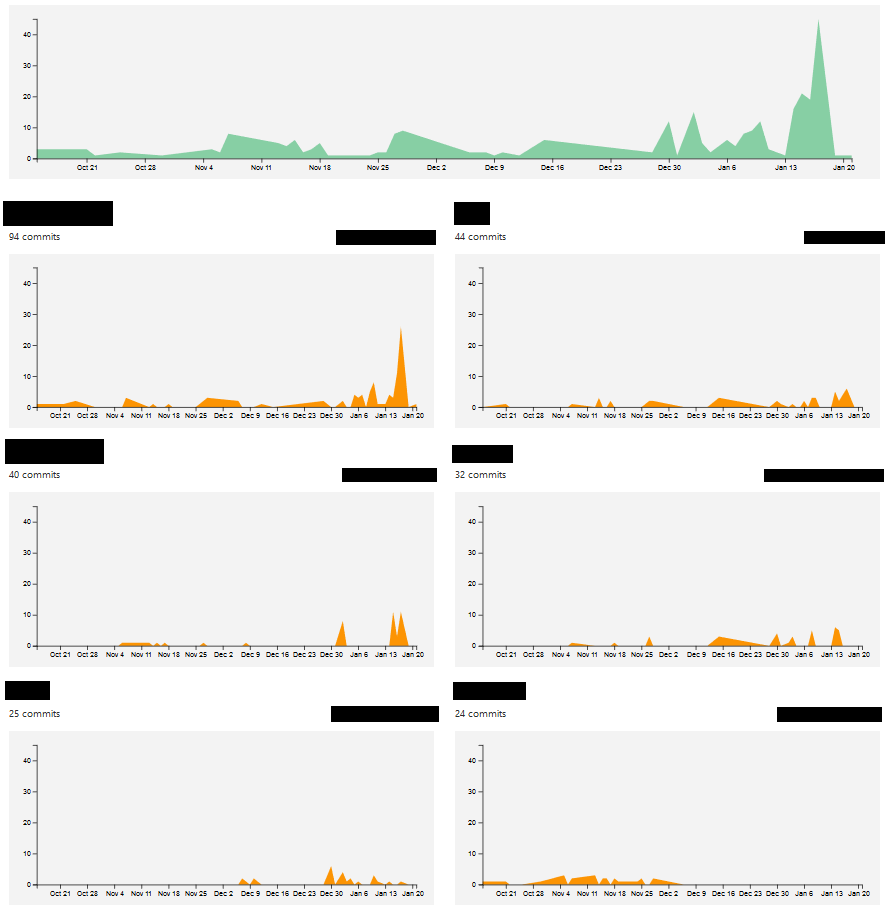
\includegraphics[scale=0.4]{slike/aktivnost.PNG} %veličina slike u odnosu na originalnu datoteku i pozicija slike
			\centering
			\caption{Primjer slike s potpisom}
			\label{fig:promjene}
		\end{figure}
		
		\begin{figure}[H]
			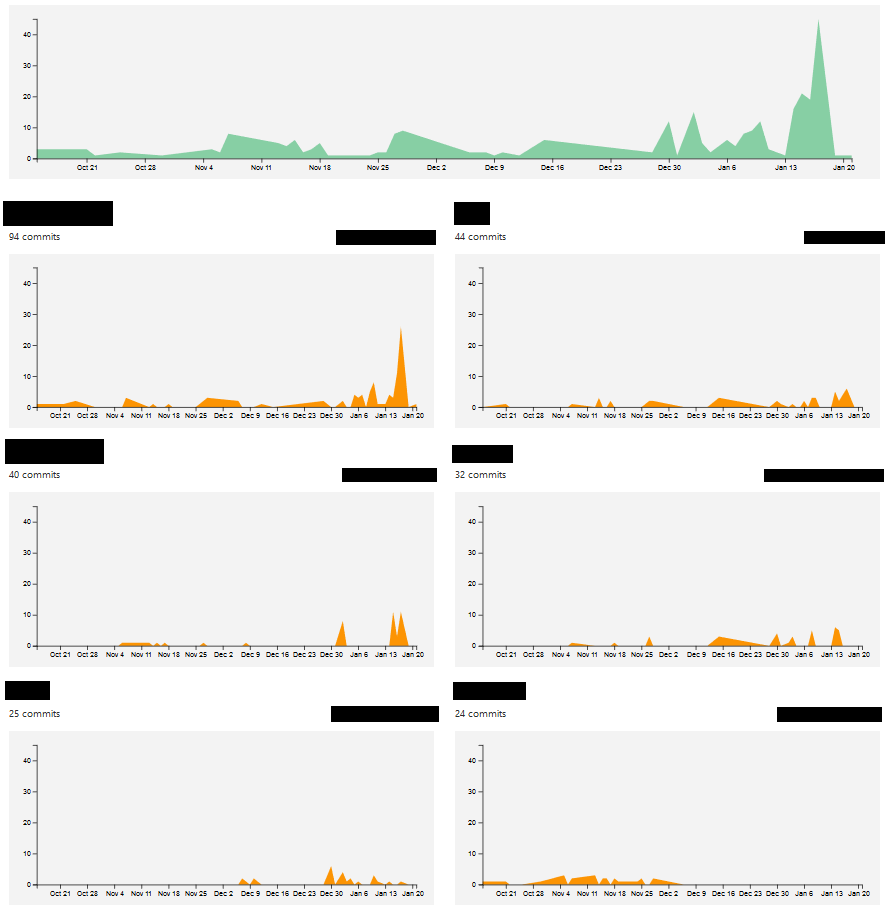
\includegraphics[width=\textwidth]{slike/aktivnost.PNG} %veličina u odnosu na širinu linije
			\caption{Primjer slike s potpisom 2}
			\label{fig:promjene2} %label mora biti drugaciji za svaku sliku
		\end{figure}
		
		Referenciranje slike \ref{fig:promjene2} u tekstu.
		
		\eject
		
	
	\chapter{Specifikacija programske potpore}
		
	\section{Funkcionalni zahtjevi}
			BRISATI KAD JE GOTOVO\\
			\textit{Navesti \textbf{dionike} koji imaju \textbf{interes u ovom sustavu} ili  \textbf{su nositelji odgovornosti}. To su prije svega korisnici, ali i administratori sustava, naručitelji, razvojni tim.}\\
				
			\textit{Navesti \textbf{aktore} koji izravno \textbf{koriste} ili \textbf{komuniciraju sa sustavom}. Oni mogu imati inicijatorsku ulogu, tj. započinju određene procese u sustavu ili samo sudioničku ulogu, tj. obavljaju određeni posao. Za svakog aktora navesti funkcionalne zahtjeve koji se na njega odnose.}\\
			KRAJ BRISANJA
			
			\noindent \textbf{Dionici:}
			
			\begin{packed_enum}
				
				\item Korisnik
				\item Administrator			
				\item Zavodi za transfuziju
				\item Hrvatski Crveni križ
				\item Razvojni tim
    
				
			\end{packed_enum}
			
			\noindent \textbf{Aktori i njihovi funkcionalni zahtjevi:}
			
			
			\begin{packed_enum}
				\item  \underbar{Neregistrirani korisnik/potencijalni donor (inicijator) može:}
				    
				\begin{packed_enum}
					
					\item pregledati potencijalne, aktivne lokacije za darivanje krvi
					\item odabrati određenu lokaciju i vidjeti generičke informacije vezane uz darivanje krvi (naziv mjesta za darivanje, adresa, telefon, OIB ustanove, slika ustanove, opće informacije darivanja krvi)
					\item pregledati trenutne zalihe krvi za različite krvne grupe u različitim centrima.
					\item registrirati se u sustav, stvoriti novi račun za koji su mu potrebni korisničko ime, lozinka, ime i prezime korisnika, OIB, adresa, broj mobitela te email adresa osobe.
				\end{packed_enum}
			
				\item  \underbar{Registrirani korisnik(potencijalni donor) može:}
				
				\begin{packed_enum}
					
					\item pregledavati svoju povijest doniranja te svoju medicinsku povijest
					\item ažurirati podatke
					\item izbrisati korisnički račun
					\item rezervirati lokaciju za doniranje krvi i pretraživati donora
					\item napisati recenziju i dati ocjenu centrima za darivanje krvi te pregledati vlastite recenzije
				\end{packed_enum}
    
                    \item  \underbar{Administrator (inicijator) može:}
				
				\begin{packed_enum}
					
					\item vidjeti popis svih registriranih korisnika i njihovih osobnih podataka
					\item brisati korisnike
					\item pristupiti statistici doniranja krvi(npr. broj darivanja krvi za određeni centar, broj ljudi s određenom krvnom grupom, povijest darivanja za određenu osobu i slično)
					\item brisati recenzije koje nisu u skladu s pravilima korištenja aplikacije
					\item dodati nove lokacije za doniranje krvi
					
				\end{packed_enum}
    
                    \item  \underbar{Baza podataka (sustav) može:}
    
                    \begin{packed_enum}
					
					\item pohranjuje sve podatke o korisnicima i njihovim ovlastima
					\item pohranjuje sve podatke o centrima darivanja krvi, njihovim kapacitetima i potrebama
					
				\end{packed_enum}
			\end{packed_enum}
			
			\eject 
			
			
				
			\subsection{Obrasci uporabe}
				
				\textbf{\textit{dio 1. revizije}}
				
				\subsubsection{Opis obrazaca uporabe}
					\textit{Funkcionalne zahtjeve razraditi u obliku obrazaca uporabe. Svaki obrazac je potrebno razraditi prema donjem predlošku. Ukoliko u nekom koraku može doći do odstupanja, potrebno je to odstupanje opisati i po mogućnosti ponuditi rješenje kojim bi se tijek obrasca vratio na osnovni tijek.}\\
					

					\noindent \underbar{\textbf{UC$<$broj obrasca$>$ -$<$ime obrasca$>$}}
					\begin{packed_item}
	
						\item \textbf{Glavni sudionik: }$<$sudionik$>$
						\item  \textbf{Cilj:} $<$cilj$>$
						\item  \textbf{Sudionici:} $<$sudionici$>$
						\item  \textbf{Preduvjet:} $<$preduvjet$>$
						\item  \textbf{Opis osnovnog tijeka:}
						
						\item[] \begin{packed_enum}
	
							\item $<$opis korak jedan$>$
							\item $<$opis korak dva$>$
							\item $<$opis korak tri$>$
							\item $<$opis korak četiri$>$
							\item $<$opis korak pet$>$
						\end{packed_enum}
						
						\item  \textbf{Opis mogućih odstupanja:}
						
						\item[] \begin{packed_item}
	
							\item[2.a] $<$opis mogućeg scenarija odstupanja u koraku 2$>$
							\item[] \begin{packed_enum}
								
								\item $<$opis rješenja mogućeg scenarija korak 1$>$
								\item $<$opis rješenja mogućeg scenarija korak 2$>$
								
							\end{packed_enum}
							\item[2.b] $<$opis mogućeg scenarija odstupanja u koraku 2$>$
							\item[3.a] $<$opis mogućeg scenarija odstupanja  u koraku 3$>$
							
						\end{packed_item}
					\end{packed_item}
				
					
				\subsubsection{Dijagrami obrazaca uporabe}
					
					\textit{Prikazati odnos aktora i obrazaca uporabe odgovarajućim UML dijagramom. Nije nužno nacrtati sve na jednom dijagramu. Modelirati po razinama apstrakcije i skupovima srodnih funkcionalnosti.}
				\eject		
				
			\subsection{Sekvencijski dijagrami}
				
				\textbf{\textit{dio 1. revizije}}\\
				
				\textit{Nacrtati sekvencijske dijagrame koji modeliraju najvažnije dijelove sustava (max. 4 dijagrama). Ukoliko postoji nedoumica oko odabira, razjasniti s asistentom. Uz svaki dijagram napisati detaljni opis dijagrama.}
				\eject
	
		\section{Ostali zahtjevi}
		
			\textbf{\textit{dio 1. revizije}}\\
		 
			 \textit{Nefunkcionalni zahtjevi i zahtjevi domene primjene dopunjuju funkcionalne zahtjeve. Oni opisuju \textbf{kako se sustav treba ponašati} i koja \textbf{ograničenja} treba poštivati (performanse, korisničko iskustvo, pouzdanost, standardi kvalitete, sigurnost...). Primjeri takvih zahtjeva u Vašem projektu mogu biti: podržani jezici korisničkog sučelja, vrijeme odziva, najveći mogući podržani broj korisnika, podržane web/mobilne platforme, razina zaštite (protokoli komunikacije, kriptiranje...)... Svaki takav zahtjev potrebno je navesti u jednoj ili dvije rečenice.}
			 
			 
			 
	
	\chapter{Arhitektura i dizajn sustava}
		
		\textbf{\textit{dio 1. revizije}}\\

		\textit{ Potrebno je opisati stil arhitekture te identificirati: podsustave, preslikavanje na radnu platformu, spremišta podataka, mrežne protokole, globalni upravljački tok i sklopovsko-programske zahtjeve. Po točkama razraditi i popratiti odgovarajućim skicama:}
	\begin{itemize}
		\item 	\textit{izbor arhitekture temeljem principa oblikovanja pokazanih na predavanjima (objasniti zašto ste baš odabrali takvu arhitekturu)}
		\item 	\textit{organizaciju sustava s najviše razine apstrakcije (npr. klijent-poslužitelj, baza podataka, datotečni sustav, grafičko sučelje)}
		\item 	\textit{organizaciju aplikacije (npr. slojevi frontend i backend, MVC arhitektura) }		
	\end{itemize}

	
		

		

				
		\section{Baza podataka}
			
			\textbf{\textit{dio 1. revizije}}\\
			
		\textit{Potrebno je opisati koju vrstu i implementaciju baze podataka ste odabrali, glavne komponente od kojih se sastoji i slično.}
		
			\subsection{Opis tablica}
			

				\textit{Svaku tablicu je potrebno opisati po zadanom predlošku. Lijevo se nalazi točno ime varijable u bazi podataka, u sredini se nalazi tip podataka, a desno se nalazi opis varijable. Svjetlozelenom bojom označite primarni ključ. Svjetlo plavom označite strani ključ}
				
				
				\begin{longtblr}[
					label=none,
					entry=none
					]{
						width = \textwidth,
						colspec={|X[6,l]|X[6, l]|X[20, l]|}, 
						rowhead = 1,
					} %definicija širine tablice, širine stupaca, poravnanje i broja redaka naslova tablice
					\hline \SetCell[c=3]{c}{\textbf{korisnik - ime tablice}}	 \\ \hline[3pt]
					\SetCell{LightGreen}IDKorisnik & INT	&  	Lorem ipsum dolor sit amet, consectetur adipiscing elit, sed do eiusmod  	\\ \hline
					korisnickoIme	& VARCHAR &   	\\ \hline 
					email & VARCHAR &   \\ \hline 
					ime & VARCHAR	&  		\\ \hline 
					\SetCell{LightBlue} primjer	& VARCHAR &   	\\ \hline 
				\end{longtblr}
				
				
			
			\subsection{Dijagram baze podataka}
				\textit{ U ovom potpoglavlju potrebno je umetnuti dijagram baze podataka. Primarni i strani ključevi moraju biti označeni, a tablice povezane. Bazu podataka je potrebno normalizirati. Podsjetite se kolegija "Baze podataka".}
			
			\eject
			
			
		\section{Dijagram razreda}
		
			\textit{Potrebno je priložiti dijagram razreda s pripadajućim opisom. Zbog preglednosti je moguće dijagram razlomiti na više njih, ali moraju biti grupirani prema sličnim razinama apstrakcije i srodnim funkcionalnostima.}\\
			
			\textbf{\textit{dio 1. revizije}}\\
			
			\textit{Prilikom prve predaje projekta, potrebno je priložiti potpuno razrađen dijagram razreda vezan uz \textbf{generičku funkcionalnost} sustava. Ostale funkcionalnosti trebaju biti idejno razrađene u dijagramu sa sljedećim komponentama: nazivi razreda, nazivi metoda i vrste pristupa metodama (npr. javni, zaštićeni), nazivi atributa razreda, veze i odnosi između razreda.}\\
			
			\textbf{\textit{dio 2. revizije}}\\			
			
			\textit{Prilikom druge predaje projekta dijagram razreda i opisi moraju odgovarati stvarnom stanju implementacije}
			
			
			
			\eject
		
		\section{Dijagram stanja}
			
			
			\textbf{\textit{dio 2. revizije}}\\
			
			\textit{Potrebno je priložiti dijagram stanja i opisati ga. Dovoljan je jedan dijagram stanja koji prikazuje \textbf{značajan dio funkcionalnosti} sustava. Na primjer, stanja korisničkog sučelja i tijek korištenja neke ključne funkcionalnosti jesu značajan dio sustava, a registracija i prijava nisu. }
			
			
			\eject 
		
		\section{Dijagram aktivnosti}
			
			\textbf{\textit{dio 2. revizije}}\\
			
			 \textit{Potrebno je priložiti dijagram aktivnosti s pripadajućim opisom. Dijagram aktivnosti treba prikazivati značajan dio sustava.}
			
			\eject
		\section{Dijagram komponenti}
		
			\textbf{\textit{dio 2. revizije}}\\
		
			 \textit{Potrebno je priložiti dijagram komponenti s pripadajućim opisom. Dijagram komponenti treba prikazivati strukturu cijele aplikacije.}
	\chapter{Implementacija i korisničko sučelje}
		
		
		\section{Korištene tehnologije i alati}
		
			\textbf{\textit{dio 2. revizije}}
			
			 \textit{Detaljno navesti sve tehnologije i alate koji su primijenjeni pri izradi dokumentacije i aplikacije. Ukratko ih opisati, te navesti njihovo značenje i mjesto primjene. Za svaki navedeni alat i tehnologiju je potrebno \textbf{navesti internet poveznicu} gdje se mogu preuzeti ili više saznati o njima}.
			
			
			\eject 
		
	
		\section{Ispitivanje programskog rješenja}
			
			\textbf{\textit{dio 2. revizije}}\\
			
			 \textit{U ovom poglavlju je potrebno opisati provedbu ispitivanja implementiranih funkcionalnosti na razini komponenti i na razini cijelog sustava s prikazom odabranih ispitnih slučajeva. Studenti trebaju ispitati temeljnu funkcionalnost i rubne uvjete.}
	
			
			\subsection{Ispitivanje komponenti}
			\textit{Potrebno je provesti ispitivanje jedinica (engl. unit testing) nad razredima koji implementiraju temeljne funkcionalnosti. Razraditi \textbf{minimalno 6 ispitnih slučajeva} u kojima će se ispitati redovni slučajevi, rubni uvjeti te izazivanje pogreške (engl. exception throwing). Poželjno je stvoriti i ispitni slučaj koji koristi funkcionalnosti koje nisu implementirane. Potrebno je priložiti izvorni kôd svih ispitnih slučajeva te prikaz rezultata izvođenja ispita u razvojnom okruženju (prolaz/pad ispita). }
			
			
			
			\subsection{Ispitivanje sustava}
			
			 \textit{Potrebno je provesti i opisati ispitivanje sustava koristeći radni okvir Selenium\footnote{\url{https://www.seleniumhq.org/}}. Razraditi \textbf{minimalno 4 ispitna slučaja} u kojima će se ispitati redovni slučajevi, rubni uvjeti te poziv funkcionalnosti koja nije implementirana/izaziva pogrešku kako bi se vidjelo na koji način sustav reagira kada nešto nije u potpunosti ostvareno. Ispitni slučaj se treba sastojati od ulaza (npr. korisničko ime i lozinka), očekivanog izlaza ili rezultata, koraka ispitivanja i dobivenog izlaza ili rezultata.\\ }
			 
			 \textit{Izradu ispitnih slučajeva pomoću radnog okvira Selenium moguće je provesti pomoću jednog od sljedeća dva alata:}
			 \begin{itemize}
			 	\item \textit{dodatak za preglednik \textbf{Selenium IDE} - snimanje korisnikovih akcija radi automatskog ponavljanja ispita	}
			 	\item \textit{\textbf{Selenium WebDriver} - podrška za pisanje ispita u jezicima Java, C\#, PHP koristeći posebno programsko sučelje.}
			 \end{itemize}
		 	\textit{Detalji o korištenju alata Selenium bit će prikazani na posebnom predavanju tijekom semestra.}
			
			\eject 
		
		
		\section{Dijagram razmještaja}
			
			\textbf{\textit{dio 2. revizije}}
			
			 \textit{Potrebno je umetnuti \textbf{specifikacijski} dijagram razmještaja i opisati ga. Moguće je umjesto specifikacijskog dijagrama razmještaja umetnuti dijagram razmještaja instanci, pod uvjetom da taj dijagram bolje opisuje neki važniji dio sustava.}
			
			\eject 
		
		\section{Upute za puštanje u pogon}
		
			\textbf{\textit{dio 2. revizije}}\\
		
			 \textit{U ovom poglavlju potrebno je dati upute za puštanje u pogon (engl. deployment) ostvarene aplikacije. Na primjer, za web aplikacije, opisati postupak kojim se od izvornog kôda dolazi do potpuno postavljene baze podataka i poslužitelja koji odgovara na upite korisnika. Za mobilnu aplikaciju, postupak kojim se aplikacija izgradi, te postavi na neku od trgovina. Za stolnu (engl. desktop) aplikaciju, postupak kojim se aplikacija instalira na računalo. Ukoliko mobilne i stolne aplikacije komuniciraju s poslužiteljem i/ili bazom podataka, opisati i postupak njihovog postavljanja. Pri izradi uputa preporučuje se \textbf{naglasiti korake instalacije uporabom natuknica} te koristiti što je više moguće \textbf{slike ekrana} (engl. screenshots) kako bi upute bile jasne i jednostavne za slijediti.}
			
			
			 \textit{Dovršenu aplikaciju potrebno je pokrenuti na javno dostupnom poslužitelju. Studentima se preporuča korištenje neke od sljedećih besplatnih usluga: \href{https://aws.amazon.com/}{Amazon AWS}, \href{https://azure.microsoft.com/en-us/}{Microsoft Azure} ili \href{https://www.heroku.com/}{Heroku}. Mobilne aplikacije trebaju biti objavljene na F-Droid, Google Play ili Amazon App trgovini.}
			
			
			\eject 
	\chapter{Zaključak i budući rad}
		
		\textbf{\textit{dio 2. revizije}}\\
		
		 \textit{U ovom poglavlju potrebno je napisati osvrt na vrijeme izrade projektnog zadatka, koji su tehnički izazovi prepoznati, jesu li riješeni ili kako bi mogli biti riješeni, koja su znanja stečena pri izradi projekta, koja bi znanja bila posebno potrebna za brže i kvalitetnije ostvarenje projekta i koje bi bile perspektive za nastavak rada u projektnoj grupi.}
		
		 \textit{Potrebno je točno popisati funkcionalnosti koje nisu implementirane u ostvarenoj aplikaciji.}
		
		\eject 
	\chapter*{Popis literature}
		\addcontentsline{toc}{chapter}{Popis literature}
	 	
 		\textbf{\textit{Kontinuirano osvježavanje}}
	
		\textit{Popisati sve reference i literaturu koja je pomogla pri ostvarivanju projekta.}
		
		
		\begin{enumerate}
			
			
			\item  Programsko inženjerstvo, FER ZEMRIS, \url{http://www.fer.hr/predmet/proinz}
			
			\item  I. Sommerville, "Software engineering", 8th ed, Addison Wesley, 2007.
			
			\item  T.C.Lethbridge, R.Langaniere, "Object-Oriented Software Engineering", 2nd ed. McGraw-Hill, 2005.
			
			\item  I. Marsic, Software engineering book``, Department of Electrical and Computer Engineering, Rutgers University, \url{http://www.ece.rutgers.edu/~marsic/books/SE}
			
			\item  The Unified Modeling Language, \url{https://www.uml-diagrams.org/}
			
			\item  Astah Community, \url{http://astah.net/editions/uml-new}
		\end{enumerate}
		
		 
	
	
	\begingroup
	\renewcommand*\listfigurename{Indeks slika i dijagrama}
	%\renewcommand*\listtablename{Indeks tablica}
	%\let\clearpage\relax
	\listoffigures
	%\vspace{10mm}
	%\listoftables
	\endgroup
	\addcontentsline{toc}{chapter}{Indeks slika i dijagrama}


	
	\eject 
		
	\chapter*{Dodatak: Prikaz aktivnosti grupe}
		\addcontentsline{toc}{chapter}{Dodatak: Prikaz aktivnosti grupe}
		
		\section*{Dnevnik sastajanja}
		
		\textbf{\textit{Kontinuirano osvježavanje}}\\
		
		 \textit{U ovom dijelu potrebno je redovito osvježavati dnevnik sastajanja prema predlošku.}
		
		\begin{packed_enum}
			\item  sastanak
			
			\item[] \begin{packed_item}
				\item Datum: u ovom formatu: \today
				\item Prisustvovali: I.Prezime, I.Prezime
				\item Teme sastanka:
				\begin{packed_item}
					\item  opis prve teme
					\item  opis druge teme
				\end{packed_item}
			\end{packed_item}
			
			\item  sastanak
			\item[] \begin{packed_item}
				\item Datum: u ovom formatu: \today
				\item Prisustvovali: I.Prezime, I.Prezime
				\item Teme sastanka:
				\begin{packed_item}
					\item  opis prve teme
					\item  opis druge teme
				\end{packed_item}
			\end{packed_item}
			
			%
			
		\end{packed_enum}
		
		\eject
		\section*{Tablica aktivnosti}
		
			\textbf{\textit{Kontinuirano osvježavanje}}\\
			
			 \textit{Napomena: Doprinose u aktivnostima treba navesti u satima po članovima grupe po aktivnosti.}

			\begin{longtblr}[
					label=none,
				]{
					vlines,hlines,
					width = \textwidth,
					colspec={X[7, l]X[1, c]X[1, c]X[1, c]X[1, c]X[1, c]X[1, c]X[1, c]}, 
					vline{1} = {1}{text=\clap{}},
					hline{1} = {1}{text=\clap{}},
					rowhead = 1,
				} 
			
				\SetCell[c=1]{c}{} & \SetCell[c=1]{c}{\rotatebox{90}{\textbf{Ime Prezime voditelja}}} & \SetCell[c=1]{c}{\rotatebox{90}{\textbf{Ime Prezime }}} &	\SetCell[c=1]{c}{\rotatebox{90}{\textbf{Ime Prezime }}} & \SetCell[c=1]{c}{\rotatebox{90}{\textbf{Ime Prezime }}} &	\SetCell[c=1]{c}{\rotatebox{90}{\textbf{Ime Prezime }}} & \SetCell[c=1]{c}{\rotatebox{90}{\textbf{Ime Prezime }}} &	\SetCell[c=1]{c}{\rotatebox{90}{\textbf{Ime Prezime }}} \\  
				Upravljanje projektom 		&  &  &  &  &  &  & \\ 
				Opis projektnog zadatka 	&  &  &  &  &  &  & \\ 
				
				Funkcionalni zahtjevi       &  &  &  &  &  &  &  \\ 
				Opis pojedinih obrazaca 	&  &  &  &  &  &  &  \\ 
				Dijagram obrazaca 			&  &  &  &  &  &  &  \\ 
				Sekvencijski dijagrami 		&  &  &  &  &  &  &  \\ 
				Opis ostalih zahtjeva 		&  &  &  &  &  &  &  \\ 

				Arhitektura i dizajn sustava	 &  &  &  &  &  &  &  \\ 
				Baza podataka				&  &  &  &  &  &  &   \\ 
				Dijagram razreda 			&  &  &  &  &  &  &   \\ 
				Dijagram stanja				&  &  &  &  &  &  &  \\ 
				Dijagram aktivnosti 		&  &  &  &  &  &  &  \\ 
				Dijagram komponenti			&  &  &  &  &  &  &  \\ 
				Korištene tehnologije i alati 		&  &  &  &  &  &  &  \\ 
				Ispitivanje programskog rješenja 	&  &  &  &  &  &  &  \\ 
				Dijagram razmještaja			&  &  &  &  &  &  &  \\ 
				Upute za puštanje u pogon 		&  &  &  &  &  &  &  \\  
				Dnevnik sastajanja 			&  &  &  &  &  &  &  \\ 
				Zaključak i budući rad 		&  &  &  &  &  &  &  \\  
				Popis literature 			&  &  &  &  &  &  &  \\  
				&  &  &  &  &  &  &  \\ \hline 
				\textit{Dodatne stavke kako ste podijelili izradu aplikacije} 			&  &  &  &  &  &  &  \\ 
				\textit{npr. izrada početne stranice} 				&  &  &  &  &  &  &  \\  
				\textit{izrada baze podataka} 		 			&  &  &  &  &  &  & \\  
				\textit{spajanje s bazom podataka} 							&  &  &  &  &  &  &  \\ 
				\textit{back end} 							&  &  &  &  &  &  &  \\  
				 							&  &  &  &  &  &  &\\ 
			\end{longtblr}
					
					
		\eject
		\section*{Dijagrami pregleda promjena}
		
		\textbf{\textit{dio 2. revizije}}\\
		
		\textit{Prenijeti dijagram pregleda promjena nad datotekama projekta. Potrebno je na kraju projekta generirane grafove s gitlaba prenijeti u ovo poglavlje dokumentacije. Dijagrami za vlastiti projekt se mogu preuzeti s gitlab.com stranice, u izborniku Repository, pritiskom na stavku Contributors.}
		
	


\end{document} %naredbe i tekst nakon ove naredbe ne ulaze u izgrađen dokument 


